% 手拉手 例1：两个等边三角形共顶点 O，顶角 60°
\documentclass[tikz,border=4pt]{standalone}
\usepackage{ctex}
\usepackage{amsmath}
\usetikzlibrary{calc, decorations.markings}
\begin{document}
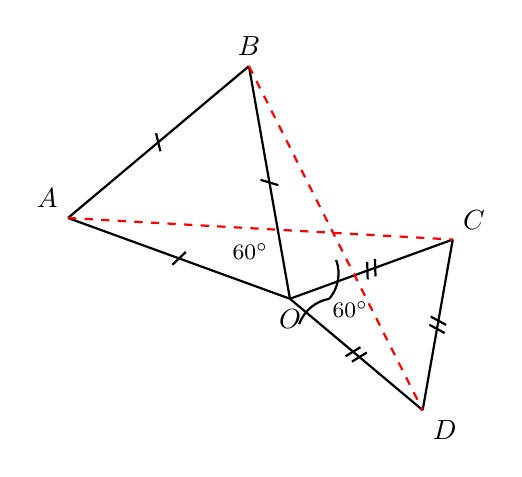
\begin{tikzpicture}[scale=1.0, thick,
  tick/.style={postaction={decorate, decoration={markings,
    mark=at position 0.5 with {\draw (-1.5pt,-3pt) -- (1.5pt,3pt);}}}},
  ticktwo/.style={postaction={decorate, decoration={markings,
    mark=at position 0.5 with {\draw (-2.5pt,-3pt) -- (-0.5pt,3pt);
                               \draw (0.5pt,-3pt)  -- (2.5pt,3pt);}}}}]
  \coordinate (O) at (0,0);
  % 等边△OAB OA=OB=3，中线方向 130°，顶角 60° => A 100°, B 160°
  \coordinate (A) at ({3*cos(160)}, {3*sin(160)});
  \coordinate (B) at ({3*cos(100)}, {3*sin(100)});
  % 等边△OCD OC=OD=2.2，中线 -10°，C 20°, D -40°
  \coordinate (C) at ({2.2*cos(20)}, {2.2*sin(20)});
  \coordinate (D) at ({2.2*cos(-40)}, {2.2*sin(-40)});

  \draw[tick] (O) -- (A);
  \draw[tick] (O) -- (B);
  \draw[tick] (A) -- (B);
  \draw[ticktwo] (O) -- (C);
  \draw[ticktwo] (O) -- (D);
  \draw[ticktwo] (C) -- (D);

  \draw (0.5,0) ++(100:0) arc[start angle=100, end angle=160, radius=0.5];
  \node at ({0.78*cos(130)},{0.78*sin(130)}) {\footnotesize $60^\circ$};
  \draw (0.5,0) ++(-40:0) arc[start angle=-40, end angle=20, radius=0.5];
  \node at ({0.78*cos(-10)},{0.78*sin(-10)}) {\footnotesize $60^\circ$};

  \draw[red, dashed] (A) -- (C);
  \draw[red, dashed] (B) -- (D);

  \node[below]       at (O) {$O$};
  \node[above left]  at (A) {$A$};
  \node[above]       at (B) {$B$};
  \node[above right] at (C) {$C$};
  \node[below right] at (D) {$D$};
\end{tikzpicture}
\end{document}
